%% MatrixLang: the paper, as submitted.
%%
%% Generated from the working draft by tools/strip_anchors.py,
%% which removes the draft's measurement-binding comments and
%% nothing else. Edit the draft, not this file.
%% MatrixLang: experience report.
%%
%% Class: acmart, sigconf. Obtain the official template from
%%   https://www.acm.org/publications/proceedings-template
%% This file references the class; it does not reproduce it.
%%
%% Build:  latexmk -pdf main.tex
%% For a double-blind venue, add `anonymous` to the class options.

\documentclass[sigconf,nonacm]{acmart}

\usepackage{booktabs}
\usepackage{graphicx}
\usepackage{listings}

\lstdefinestyle{ml}{
  basicstyle=\ttfamily\scriptsize,
  keywordstyle=\bfseries,
  commentstyle=\itshape\color{gray},
  morekeywords={matrix,scalar,print,transpose,identity,zeros,ones},
  morecomment=[l]{//},
  morecomment=[s]{/*}{*/},
  columns=fullflexible,
  keepspaces=true,
  showstringspaces=false,
  aboveskip=4pt, belowskip=2pt,
}
\lstset{style=ml}

\begin{document}

\title{Shapes in the Type System}
\subtitle{A Matrix Language That Lets a Compiler Course Reach Optimization}

\author{A Aswanth Raj}
\affiliation{%
  \institution{Compiler Design Laboratory}
  \country{India}
}

%% ------------------------------------------------------------------ abstract
\begin{abstract}
A compiler-construction project is usually built for a subset of C, and the
choice is rarely examined. In such a language the type system is a small
enumeration, so semantic analysis reduces to comparing two tags and the
optimizer has only scalar identities to work with.

We report on MatrixLang, a language whose types carry matrix shapes, used for a
one-semester compiler project. Every shape is known at compile time, so the
compiler can cost a program before it runs, and can choose the bracketing of a
matrix product chain. We measure the consequences on 400 generated programs.
Optimized and unoptimized execution agree byte for byte on all of them.
The optimizer removes a median of 48.5\% of the arithmetic (IQR 2.5 to 81.7).
On the same programs, measured the conventional way instead, it removes 5.6\% of
the instructions (IQR 0.0 to 9.1): the same optimizer, scored on a quantity it
was never built to reduce.

An instruction count therefore understates the effect roughly ninefold, and
differential testing over the same corpus found a real defect in our own
optimizer. MatrixLang reaches all eight canonical phases; three public C-subset
course compilers reach five, three and six, and none contains an optimizer. We
claim reachability, not a learning outcome: the language has not been taught.
\end{abstract}

\keywords{compiler construction, computing education, domain-specific languages,
type systems, code optimization}

\maketitle

%% ------------------------------------------------------------- introduction
\section{Introduction}

Ask what a compiler-construction course project should compile and the usual
answer is a subset of C. Lab manuals specify it, textbooks assume it, and the
public repositories students leave behind confirm it. Nobody argues for it,
because nobody has to.

The choice is defensible, and it is almost never examined, which is a pity,
because its consequence for the rest of the course is not small.
A subset of C has perhaps two numeric types, so its type system
is an enumeration with two members. Semantic analysis over such a type system is
a comparison of two tags. An optimizer over it has constant folding and the
scalar identities, none of which involve anything the front end had to work to
discover. The two phases that the syllabus presents as the intellectual centre
of the subject become, in the project, the two phases with the least to do.

This paper reports what happened when we changed the source language instead of
the curriculum. MatrixLang is a small imperative language whose values are
scalars and matrices, and whose types carry matrix shape: a value is not of type
\texttt{matrix} but of type \texttt{Matrix<2x3>}. Nothing about that idea is new,
and we claim nothing about it (Section~\ref{sec:related}). What we report is
what it made reachable in a course project, and what we measured once it was.

\paragraph{Contributions.}
\begin{enumerate}
\item An account of a shape-typed matrix language used as a compiler-course
      vehicle, with the design decisions that kept it within one semester
      (Section~\ref{sec:lang}).
\item The observation that shape information is a \emph{cost model} as well as a
      correctness device, which lets a teaching optimizer be scored in
      arithmetic removed rather than instructions removed
      (Section~\ref{sec:cost}).
\item Measurements on 400 randomly generated programs showing that the two
      metrics disagree by roughly nine times, that chain re-bracketing helps
      about 80\% of programs while leaving the instruction count untouched, and
      that optimized and unoptimized execution agree everywhere
      (Section~\ref{sec:eval}).
\item A phase-by-phase comparison against three public C-subset course
      compilers, none of which contains an optimizer
      (Section~\ref{subsec:baselines}).
\item A defect our own differential testing found: an algebraic rewrite that is
      valid over the reals and unsound under IEEE-754 signed zero
      (Section~\ref{subsec:differential}).
\end{enumerate}

%% ------------------------------------------------------------------ related
\section{Background and Related Work}
\label{sec:related}

\paragraph{Domain-specific languages in compiler courses.}
Henry~\cite{henry2005teaching} argues that building a compiler for a
domain-specific language engages students more than a conventional project,
and reports using one in an upper-division course. That argument is about
engagement. Ours is about which phases can carry content: a different claim
about the same choice. Chakraborty et al.~\cite{chakraborty2011practicum}
describe a compiler-construction practicum, and the scope problem a semester
imposes on one. Abounegm et al.~\cite{abounegm2024stella} present Stella, a
purpose-built extensible language for teaching type-system implementation, and
report student outcomes; Stella targets type systems in a course that already
assumes compiler basics, and makes no argument about source-language choice
across the pipeline.

\paragraph{Shapes in types.}
Static shape checking for matrix and tensor programs is an established and
active area, from dependent and refinement types through to shape-typed
intermediate representations in deep-learning compilers. MatrixLang's type
system is the simplest thing in that space that works, and is not offered as a
contribution.

\paragraph{Linear-algebra compilers.}
Linnea~\cite{barthels2021linnea} generates efficient linear-algebra programs,
costing candidate kernel sequences in floating-point operations and selecting
among them, with a property inference engine covering identity, diagonal,
triangular, symmetric, positive-definite and orthogonal operands. LGen and its
structured-matrix successor~\cite{spampinato2014lgen,spampinato2016structured}
compile fixed-size linear-algebra expressions to vectorised code. Everything
MatrixLang's optimizer does, these systems do more thoroughly. Our cost model is
the textbook $m p (2n-1)$ and our chain ordering is the textbook $O(k^3)$
dynamic program, chosen in both cases because they are teachable in a lecture.
The distinction we draw is one of purpose: those are production code generators
evaluated against numerical libraries, and this is a course project evaluated on
what a student can build and measure.

\paragraph{Floating point.}
That identities valid over the reals are unsound over IEEE-754 is textbook
material~\cite{goldberg1991floating}, and production compilers gate the affected
rewrites behind unsafe-math options for exactly this reason. We claim no finding
about arithmetic; we report that a course-scale testing setup rediscovered one of
these hazards in our own code.

%% ------------------------------------------------------------------ language
\section{MatrixLang}
\label{sec:lang}

MatrixLang is imperative and deliberately small. A program is a sequence of
declarations, assignments and prints:

\begin{lstlisting}
matrix A[2,3] = {{1, 2, 3},
                 {4, 5, 6}};
matrix B[3,4];
matrix C = A * B;      // shape inferred: Matrix<2x4>
print(C);
\end{lstlisting}

There are two kinds of value, scalars and matrices, and the type of a matrix
carries its shape. \texttt{Matrix<2x3>} and \texttt{Matrix<3x2>} are different
types. Operations are $+$, $-$, $*$, unary $-$ and \texttt{transpose}, with
\texttt{identity}, \texttt{zeros} and \texttt{ones} as constructors. Every shape
rule lives in one 108-line file, consulted by both the semantic analyser and the
code generator, so there is exactly one place that decides whether $A * B$ is
legal and what shape it produces.

Two design decisions shaped the project more than any other.

\paragraph{There is no control flow.}
MatrixLang has no \texttt{if} and no loops. The immediate consequence is that a
program is a single basic block, so available-expression analysis and liveness
are each one linear scan. A course reaches working common-subexpression
elimination and dead-code elimination without first building a control-flow
graph and an iterative dataflow framework. We offer this as a design rationale
rather than a result: we have not measured student time against a
control-flow-bearing alternative, and Section~\ref{sec:limits} says so.

\paragraph{Constructors exist so the optimizer can see properties.}
\texttt{identity(n)} and \texttt{zeros(r,c)} are not conveniences. An optimizer
can only fold $A \cdot I$ away if it knows some value \emph{is} an identity, and
a shape does not tell it that: \texttt{Matrix<3x3>} is consistent with any
$3\times3$ matrix. The optimizer therefore tracks a small property lattice alongside the shape
(identity, zero matrix, scalar one, scalar zero, and ``is the transpose of
$x$''), propagating it through copies and
invalidating it on redefinition. Matrix literals are inspected for the same
properties, so a hand-written $\{\{1,0\},\{0,1\}\}$ folds exactly as
\texttt{identity(2)} does.

The compiler is 4{,}700 lines of C organised by phase, with Flex and Bison for
the front end and no other dependency. It exposes one flag per phase
(\texttt{--tokens}, \texttt{--ast}, \texttt{--symbols}, \texttt{--tac},
\texttt{--optimize}, \texttt{--target}, \texttt{--run}), which turns assessment
from reading source into running the tool.

%% ---------------------------------------------------------------- cost model
\section{Shape Information as a Cost Model}
\label{sec:cost}

The observation this paper is built around is that a shape known at compile time
fixes arithmetic cost at compile time.

The product of an $m \times n$ matrix with an $n \times p$ matrix performs
$m p n$ multiplications and $m p (n-1)$ additions. Every term is a shape, and in
MatrixLang every shape is in the type. The compiler can therefore report exactly
how much arithmetic a program will perform before it runs, and an optimizer can
be scored on arithmetic removed rather than on lines removed.

That distinction matters more than it first appears. Removing one instruction
that multiplies two $200\times200$ matrices is worth vastly more than removing
three that add $2\times2$ ones, and an instruction count cannot tell them apart.
Worse, an instruction count is easy to flatter: an example written so that many
instructions vanish produces a good percentage.

\paragraph{Chain ordering.}
The optimization this makes possible is the one a scalar compiler cannot express
at all. Matrix multiplication is associative, so $A \cdot B \cdot C$ may be
bracketed either way and both compute the same matrix. They do not perform the
same arithmetic. With $A$ of shape $100\times2$, $B$ of $2\times100$ and $C$ of
$100\times2$:

\begin{center}
\begin{tabular}{@{}lr@{}}
\toprule
bracketing & arithmetic \\
\midrule
$(A \cdot B) \cdot C$ & 69{,}800 FLOP \\
$A \cdot (B \cdot C)$ &  1{,}396 FLOP \\
\bottomrule
\end{tabular}
\end{center}

The source says $A * B * C$ and $*$ is left-associative, so the program as
written asks for the first. The compiler chooses the second, by the standard
$O(k^3)$ dynamic program over the shapes. A chain of $k$ matrices needs exactly
$k-1$ products under every bracketing, so this transformation \emph{never
changes the instruction count} --- on this example it removes 98.0\% of the
arithmetic while leaving the instruction count at four.

%% --------------------------------------------------------------- evaluation
\section{Evaluation}
\label{sec:eval}

Every example program in the repository was written by the same person who wrote
the optimizer, which makes any percentage taken over them circular: the examples
that exercise a pass exist because the pass exists. All measurements below are
taken on programs produced by a generator instead.

The generator builds programs shape-correct by construction, assembling
expressions from operands whose shapes already agree, and draws the shapes
themselves at random. Dimensions are drawn from
$\{1,2,3,5,8,12,20,32,50,80,120,200\}$ for cost measurement and from $1..4$ for
execution. Products and chains are weighted to dominate the expression mix.
Everything is reproducible from a recorded seed. We report two seeds of 200
programs each and do not pool them, so the replication is visible.

\subsection{Does optimization preserve meaning?}
\label{subsec:differential}

Each generated program is executed twice, with the optimizer and without, and
the outputs compared byte for byte. Across both seeds, 400 of 400 programs agree.

That result is only interesting because the first run did not.
One program in the first 200 disagreed: it printed \texttt{0} unoptimized and
\texttt{-0} optimized. The cause was an algebraic rewrite in our own optimizer,
$0 - x \Rightarrow -x$. The identity holds over the reals. It does not preserve
observable behaviour in IEEE-754, because $+0 - +0$ evaluates to $+0$ while
negating $+0$ gives $-0$, and the two print differently. We removed the rewrite;
it saves no arithmetic, since a negation costs what a subtraction from zero
costs.

We draw two things from this. The hazard itself is textbook, and we claim
nothing about it. What is worth reporting is that a testing setup of a size a
course project can build, a generator and a loop comparing two runs, found a
defect in a student-scale optimizer that code review had not, on an input
nobody had chosen. Over the author-written example corpus the same check passes, and passing
there demonstrates only that the code runs.

\subsection{Arithmetic against instructions}

\begin{figure}[t]
\centering
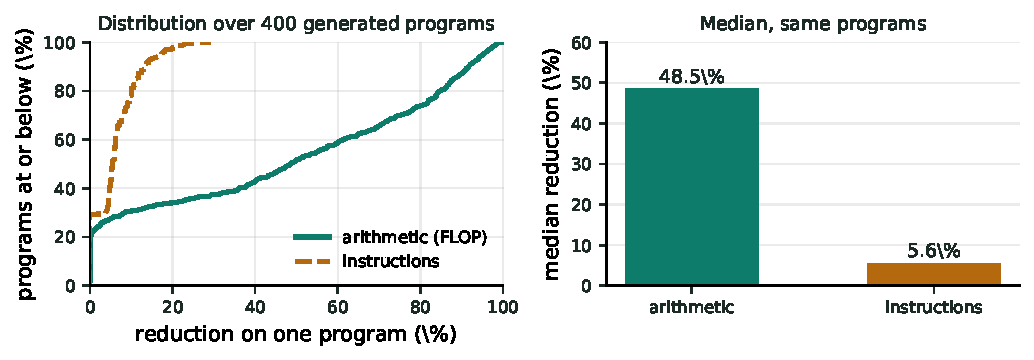
\includegraphics[width=\columnwidth]{figures/reduction.pdf}
\caption{What the optimizer removes from 400 generated programs, by each metric.
Left: the cumulative distribution of per-program reduction. Right: the medians,
over the same programs.}
\label{fig:reduction}
\end{figure}

Measured both ways on the same programs, the optimizer removes
a median of 48.5\% of the arithmetic (IQR 2.5 to 81.7).
It removes a median of 5.6\% of the instructions (IQR 0.0 to 9.1).

Figure~\ref{fig:reduction} shows the two distributions, and
Table~\ref{tab:seeds} gives the figures at each seed separately. The gap is
not an artifact of the median: the arithmetic curve lies above the instruction
curve across its whole range, and the direction is the same at both seeds.

\begin{table}[t]
\caption{Per-program reduction, by corpus and by metric. Each figure is a
median over the programs in that row, with its interquartile range beside it.
The two seeds are independent corpora of 200 programs each; pooled is all 400.}
\label{tab:seeds}
\small
\begin{tabular}{lll}
\toprule
corpus & arithmetic removed & instructions removed \\
\midrule
first seed & 47.3\% (IQR 1.1 to 78.3) & 5.3\% (IQR 0.0 to 9.2) \\
second seed & 49.7\% (IQR 2.7 to 82.2) & 5.9\% (IQR 0.0 to 9.1) \\
\addlinespace
pooled & 48.5\% (IQR 2.5 to 81.7) & 5.6\% (IQR 0.0 to 9.1) \\
\bottomrule
\end{tabular}
\end{table}

The reason is structural rather than incidental. Most of what the optimizer
removes is expensive work rather than many lines, and the largest single
contributor, chain re-bracketing, removes no lines at all by construction.
An optimizer scored in instructions is being scored on a quantity it was not
built to reduce.

\subsection{How often does bracketing matter?}

Chain re-bracketing changes something on 79.8\% (Wilson 95\% CI 75.5 to 83.4) of generated programs, 319 of 400.
On those it removes a median of 60.1\% of the arithmetic (IQR 26.2 to 84.0).

The two corpora agree closely. At the first seed it is 79.5\%, 159 of 200 (Wilson 95\% CI 73.4 to 84.5).
At the second it is 80.0\%, 160 of 200 (Wilson 95\% CI 73.9 to 85.0).

Roughly a fifth of programs are left alone, and they belong in the table.
When the shapes make left-to-right the cheapest bracketing, the dynamic program
says so and the compiler does nothing. Twenty-seven programs at
the first seed saw no arithmetic reduction from any pass at all. An optimizer
that always reports an improvement is not measuring anything.

\subsection{What the baselines reach}
\label{subsec:baselines}

MatrixLang reaches 8 of 8 canonical phases; the baselines reach 5, 3 and 6.
We cloned three public repositories that describe themselves as compiler-design
course projects for a subset of C built with Lex and Yacc, selected by that
description before their contents were inspected, and searched each for markers
of the eight canonical phases. A single case-insensitive mention counts as
present, which is generous to the baselines. No tuning or configuration was
applied to any repository: the comparison is of what each contains, not of how
well any of them performs.

\begin{table}[t]
\caption{Compiler phases for which a marker was found. Three public C-subset
course projects, and MatrixLang.}
\label{tab:phases}
\small
\begin{tabular}{@{}lcccc@{}}
\toprule
phase & ML & B1 & B2 & B3 \\
\midrule
lexical analysis        & \checkmark & \checkmark & \checkmark & \checkmark \\
syntax analysis         & \checkmark & \checkmark & \checkmark & \checkmark \\
symbol table            & \checkmark & \checkmark &            & \checkmark \\
semantic analysis       & \checkmark & \checkmark &            & \checkmark \\
intermediate code       & \checkmark &            & \checkmark & \checkmark \\
code optimization       & \checkmark &            &            &            \\
target code generation  & \checkmark & \checkmark &            & \checkmark \\
execution               & \checkmark &            &            &            \\
\midrule
total                   & 8 & 5 & 3 & 6 \\
\bottomrule
\end{tabular}
\end{table}

Table~\ref{tab:phases} gives the result. MatrixLang reaches all eight. The
baselines reach five, three and six, and \emph{none of the three contains an
optimizer or an execution engine}: all stop at intermediate code generation.

This is an existence result at $n=3$ on a convenience sample, and we report it
as one. It does not establish a proportion over what courses assign. It does
establish that the pattern the design was aimed at is real in practice, and it
is consistent with what the scope discussion in the pedagogy literature would
predict.

%% --------------------------------------------------------------- discussion
\section{Discussion}

\paragraph{What the domain bought.}
Three phases gained content that a C-subset project does not give them.
\emph{Semantic analysis} became shape inference: the analyser computes the shape
of every expression and rejects the operations whose shapes do not combine, with
a diagnostic naming both operands, the rule, and the values found. \emph{Code
generation} gained instruction selection, because one source-level \texttt{*}
becomes a matrix product, a scaling or a scalar multiply depending only on
inferred types. \emph{Optimization} gained transformations with a measurable
effect and a cost model to measure them with.

\paragraph{What it cost.}
The language has no control flow, so the project does not teach control-flow
graphs or iterative dataflow analysis, which a C-subset project can. This is a
real trade and we do not think it is free. Our position is that a course reaching
a working optimizer over straight-line code teaches more about optimization than
one that builds a CFG and runs out of semester before using it, but we have not
tested that position.

\paragraph{On measuring optimizers in a course.}
The wider transferable point does not depend on matrices. Whatever the domain,
if the type system carries enough information to cost a program statically, a
student's optimizer can be evaluated on work removed rather than lines removed,
and the two are not close. We would expect the same argument to apply to a
language over units, over relational algebra, or over fixed-size vectors.

%% -------------------------------------------------------------- limitations
\section{Limitations}
\label{sec:limits}

\emph{It has not been taught.} MatrixLang was built as a project, not yet
deployed as one. We claim what the design makes reachable; we make no claim
about learning, retention, or student time, and we have no student data.

\emph{The corpus is synthetic.} The generator was written for this project, so
the distribution of shapes and expression forms is a choice rather than a sample
of real MatrixLang programs, and no such sample can exist for a new language.
The direction of the cost-versus-instruction result does not depend on that
choice.
The magnitude is not, and should be read as a property of this corpus.

\emph{The baseline sample is small.} Three repositories, chosen by search
description, all from one hosting site.

\emph{The cost model is a model.} It counts scalar arithmetic and ignores memory
traffic, cache behaviour and parallelism, all of which dominate real runtimes.
It is the right measure for what an optimizer removed and the wrong one for how
fast the result runs.

%% -------------------------------------------------------------- conclusion
\section{Conclusion}

The source language of a compiler project is a curricular decision, and it
decides which phases can carry real work. A subset of C leaves semantic analysis
and optimization with little to do, which is visible in the public record: of
three C-subset course compilers we measured, none contains an optimizer.

Putting matrix shapes into the type system changes that, because a shape is both
a correctness device and a cost model. The resulting course project reaches all
eight canonical phases, and its optimizer can be scored honestly. Over 400
programs an instruction count reports a median reduction of 5.6\% (IQR 0.0 to 9.1).
The arithmetic actually removed is a median of 48.5\% (IQR 2.5 to 81.7).

Whether students learn more this way is the obvious next question and the one we
cannot yet answer. The compiler, the generator and the measurement scripts are
available so that someone teaching a course can find out.

%% ------------------------------------------------------------- statements
\section*{Data and Code Availability}

Code availability: the compiler, the program generator and the measurement
scripts are in the project repository. Data availability: the recorded
experiment output is in the same repository. Every figure and table in this
paper is regenerated from that recorded output rather than transcribed, and the
generated corpora are reproducible from the seeds given.

\section*{Funding}

This work received no external funding.

\section*{Conflicts of Interest}

The author declares no competing interests, financial or otherwise.

\section*{Ethics Statement}

No human participants took part and no personal data was collected. The study
measures source code, some of it from public repositories, used as published.

%% ---------------------------------------------------------- AI disclosure
\section*{Use of AI Assistance}

An AI coding assistant was used during implementation, literature search and
drafting. All design decisions, measurements and claims were reviewed and
validated by the author, who is responsible for the content of this paper.

\section*{Reproducibility Checklist}

Each result in this paper can be regenerated from the repository with a
single command, and no number in it was transcribed by hand.

\begin{itemize}
\item \emph{Corpora.} \texttt{tools/gen\_programs.py} writes the generated
      programs. Output depends only on the seed; seeds 1 and 2 are reported.
\item \emph{Measurements.} \texttt{tools/run\_experiments.py} runs the
      differential, cost and chain experiments and writes per-program JSON.
\item \emph{Figure~\ref{fig:reduction}.} \texttt{tools/plot\_reduction.py}
      draws it from that JSON.
\item \emph{Table~\ref{tab:phases}.} \texttt{tools/compare\_baselines.py}
      records its selection rules and marker list in its own output.
\end{itemize}

%% ------------------------------------------------------------- bibliography
\begin{thebibliography}{9}

\bibitem{henry2005teaching}
Tyson R. Henry. 2005.
\newblock Teaching compiler construction using a domain specific language.
\newblock In \emph{Proceedings of the 36th SIGCSE Technical Symposium on
Computer Science Education}.
\newblock DOI: 10.1145/1047344.1047364

\bibitem{chakraborty2011practicum}
Pinaki Chakraborty, P. C. Saxena, C. P. Katti, Gauri Pahwa, and Shweta Taneja.
2011.
\newblock A new practicum in compiler construction.
\newblock \emph{Computer Applications in Engineering Education}.
\newblock DOI: 10.1002/cae.20566

\bibitem{abounegm2024stella}
Abdelrahman Abounegm, Nikolai Kudasov, and Alexey Stepanov. 2024.
\newblock Teaching Type Systems Implementation with Stella, an Extensible
Statically Typed Programming Language.
\newblock In \emph{Trends in Functional Programming in Education (TFPIE 2024)},
EPTCS 405.
\newblock arXiv: 2407.08089

\bibitem{barthels2021linnea}
Henrik Barthels, Christos Psarras, and Paolo Bientinesi. 2021.
\newblock Linnea: Automatic Generation of Efficient Linear Algebra Programs.
\newblock \emph{ACM Transactions on Mathematical Software} 47, 3.
\newblock DOI: 10.1145/3446632

\bibitem{spampinato2014lgen}
Daniele G. Spampinato and Markus P\"uschel. 2014.
\newblock A Basic Linear Algebra Compiler.
\newblock In \emph{Proceedings of the Annual IEEE/ACM International Symposium on
Code Generation and Optimization}.
\newblock DOI: 10.1145/2544137.2544155

\bibitem{spampinato2016structured}
Daniele G. Spampinato and Markus P\"uschel. 2016.
\newblock A basic linear algebra compiler for structured matrices.
\newblock In \emph{Proceedings of the 2016 International Symposium on Code
Generation and Optimization}.
\newblock DOI: 10.1145/2854038.2854060

\bibitem{goldberg1991floating}
David Goldberg. 1991.
\newblock What every computer scientist should know about floating-point
arithmetic.
\newblock \emph{ACM Computing Surveys} 23, 1, 5--48.
\newblock DOI: 10.1145/103162.103163

\end{thebibliography}

\end{document}
